\graphicspath{{chapters/background/}}


\chapter{Background: Multiview Machine Learning: Concepts, Methods, and Limitations}\label{ch:background}
 \epigraph{Principal Component Analysis is a dimensionally invalid method that gives people a delusion that they are doing something useful with their data. If you change the units that one of the variables is measured in, it will change all the “principal components”! It’s for that reason that I made no mention of PCA in my book.}{Professor David MacKay}
\minitoc

\section{Introduction}

This chapter provides the foundational knowledge needed to understand the thesis as a whole, while the individual chapters will provide more specific background information as needed.

\section{Machine Learning and Multiview Learning}

Machine learning encompasses methods that enable models to learn patterns and make decisions from data. Machine learning methods are typically categorized by a training set of data, which is used to learn a model, and a test set of data, which is used to evaluate the model.

Arguably the most common machine learning paradigm is supervised learning, where the training data consists of pairs of inputs and outputs, and the model learns to predict a function that maps the inputs to the outputs. This function is then used to predict the outputs for new inputs. The goal of supervised learning is to learn a function that generalizes well to new data, i.e., to make accurate predictions on unseen data.
At the heart of many machine learning algorithms lies the concept of representation learning - the process of automatically discovering and extracting meaningful features or \gls{representations} from raw data. Representation learning aims to transform high-dimensional, complex data into a lower-dimensional space that captures the most salient aspects of the original data. This process not only reduces computational complexity but also uncovers hidden structures and relationships within the data, which can then be leveraged for various tasks such as classification, regression, or clustering.

Unsupervised and self-supervised learning are common machine learning paradigms that often involve learning low-dimensional \textit{latent} \gls{representations} of the input data. In these paradigms, the training data consists of inputs only, and the model learns to find patterns or structure in the data without explicit output labels. \textit{Downstream} models can use these learned \gls{representations} as their inputs rather than the original data.

While the distinction between unsupervised and self-supervised learning is sometimes blurred, unsupervised learning has typically been used to describe dimensionality reduction, clustering, and generative modeling algorithms. Self-supervised learning (SSL) describes a special case of unsupervised learning where the system derives \textit{labels} from the data itself \citep{balestriero2023cookbook}. The cornerstone of SSL is the concept of a \textit{pretext task}, a learning task created from the data that trains the model to capture useful features or representations. Most famously, SSL is the backbone to the success of Large Language Models \citep{vaswani2017attention} and in particular ChatGPT \citep{chatgpt}, a language model trained on a pretext task of predicting masked words in a sentence. SSL methods have also recently been shown to outperform supervised methods for certain computer vision tasks for large datasets \citep{goyal2019scaling}.


\subsection{Multiview Machine Learning}
This thesis is focussed on multiview machine learning.
Here, data from different sources or modalities, referred to as \gls{views}, such as neuroimaging, genomics, and clinical records, are analyzed collectively to unveil underlying patterns.
Multiview machine learning encompasses a variety of techniques aimed at learning from data that have multiple sources or modalities, also known as \gls{views}.
These techniques broadly fall into categories of supervised and self-supervised multiview learning, with some algorithms straddling the boundary between the two.

\subsubsection{Supervised Multiview Learning}

In supervised multiview learning, the goal is to fuse information from multiple distinct \gls{views} or feature sets to improve the predictive performance of a model. This approach involves integrating the various views, often using one view as the target variable and the others as predictors. The model learns to combine the information from the different \gls{views} to make more accurate predictions than would be possible using any single view alone.

For instance, in the context of mental health, we can consider behavioral data as a dependent variable influenced by multiple independent variables like brain activity and demographics. Figure \ref{fig:mentalhealthsupervised} illustrates this concept, where behavioral patterns ($y_1$) are predicted based on features from brain activity ($x_1$) and demographic information ($x_2$). The model learns to fuse the information from the brain and demographic \gls{views} to form a more comprehensive understanding of the factors influencing behavior.

\begin{figure}
    \centering
    \tikz{
    % nodes
        \node[obs, minimum size=3cm, align=center] (y1) {Behaviour\\$y_1$}; % Behaviour node as y1
        \node[obs, left=of y1, minimum size=3cm, align=center] (x1) {Brain\\$x_1$}; % Brain node as x1
        \node[obs, below=of x1, minimum size=3cm, align=center] (x2) {Demographics\\$x_2$};
        \edge{x1} {y1}
        \edge{x2} {y1}}
        \caption[Supervised multiview learning in mental health]{\textit{\textbf{Supervised multiview learning in mental health:}} An example of how different \gls{views} (brain activity and demographics) can be fused to predict a target variable (behavior) in a supervised learning setting.}\label{fig:mentalhealthsupervised}
\end{figure}

Multiple Kernel Learning (MKL) \citep{gonen2011multiple} is a prominent example of supervised multiview learning, where the algorithm learns to combine kernel \gls{representations} of the different views. By fusing the information from the various kernels, MKL enhances the model's predictive capabilities compared to using a single kernel.

With the advent of deep learning, the underlying concept of MKL has been extended to deep learning architectures. These architectures enable the model to learn and fuse \gls{representations} from various \gls{views} more effectively \citep{guo2019deep}. The deep learning models can automatically learn the most informative features from each view and combine them in non-linear ways to make predictions.

I contributed to this line of research through the software package Fusili \citep{florence_townend_2023_10228564}, which implements a number of deep-learning based multi-modal data fusion methods for supervised learning. Fusili provides a flexible framework for building models that can fuse information from various data modalities, such as images, text, and structured data, to make more accurate predictions.

In summary, supervised multiview learning involves fusing information from multiple \gls{views} to improve predictive performance. By combining the unique perspectives offered by each view, these methods can form a more comprehensive understanding of the problem and make more accurate predictions than would be possible using any single view alone.

\subsubsection{Self-Supervised Multiview Learning}

In contrast to supervised multiview learning, where explicit labels guide the learning process, self-supervised multiview learning operates under the hypothesis that different \gls{views} are manifestations of a shared, yet hidden, latent variable \citep{zong2023self}.
This approach, as evidenced in the latent variable model of mental health illustrated in Figure \ref{fig:mentalhealthselfsupervised}, suggests that both neuroimaging and behavioural data are influenced by an underlying factor, such as the severity of a mental health condition, which remains unobserved.

\begin{figure}
    \centering
    \tikz{
    % nodes
        \node[latent, align=center, minimum size=2cm] (Z) {Severity\\z};
        %
        \node[obs, below left=of Z, minimum size=2cm, align=center] (x1) {Brain\\$x^{(1)}$};
        \node[obs, below right=of Z, minimum size=2cm, align=center] (x2) {Behaviour\\$x^{(2)}$};
        % edges
        \edge{Z} {x1}
        \edge{Z} {x2}}
    \caption[Latent Variable Model of Mental Health]{\textit{\textbf{Latent Variable Model of Mental Health:}} From this perspective the neuroimaging modality and behavioural data are both considered to have been generated with distributions conditioned on the severity of a mental health condition}\label{fig:mentalhealthselfsupervised}
\end{figure}

A key challenge in self-supervised learning is designing pretext tasks to estimate this latent source from the available views.
A common approach is to estimate a common low-dimensional representation of the variance in the data from both \gls{views}.
In most objectives of this form, this ammounts to identifying the mutual information between the \gls{views}.
These \gls{representations} may be informative for their own sake, identifying common factors between the \gls{views}, or they may be used as inputs to a downstream task, such as classification or regression.

\subsection{Conditional Independence, Causality, and Multiview Learning}

The graphical model in Figure \ref{fig:mentalhealthsupervised} represents the assumption that the brain and demographics are independent variables, and that the behaviour is a conditional variable, dependent on both the brain and demographics.

On the other hand, the graphical model in Figure \ref{fig:mentalhealthselfsupervised} represents the assumption that the brain and behaviour are conditionally independent given the severity of an unobserved latent mental health condition.

\citet{reichenbach1956direction} introduced the epoynmous Reichenbach's principle, which states that if two variables are correlated, then either one causes the other, or both are caused by a third variable.
While the relationship between conditional independence and causality is nuanced \citep{pearl2009causality}, it is clear that our assumptions about the causal structure of the data can inform our choice of multiview learning algorithm.
In particular, we could envision a number of causal structures that could give rise to the observed data in Figure \ref{fig:mentalhealthselfsupervised}:

\begin{itemize}
    \item direct causation (brain influencing behavior or vice versa or even both)
    \item both being influenced by a common, possibly unobserved, cause
    \item no direct causal link between them
\end{itemize}

In the first case, we might be more inclined to use a supervised multiview learning algorithm to predict one view from the other.
In the second case, we might be more inclined to use a self-supervised multiview learning algorithm to estimate the latent variable.

\subsubsection{Complementary and Redundant Information}
The nature of the information provided by different \gls{views} (such as neuroimaging and behavioral data) is important for understanding multiview learning models.
A particularly useful distinction is between complementary and redundant information \citep{nguyen2020multiview,lyu2021understanding, chen2022representation}.
The complementary information in \gls{views} offers unique insights into different aspects of the same subject. For instance, in mental health studies, neuroimaging might reveal structural changes in the brain that are not (yet) present in presented behavioural phenotypes, while behavioral data could be influenced by demographic factors that do not present as structural differences in the brain. Both these \gls{views} together provide a more holistic understanding of a mental health condition.
Conversely, redundant information in different \gls{views} refers to overlapping or similar data presented from various angles. For instance, a specific mental health condition may manifest in both observable behavioral changes and detectable neuroimaging markers. While each view alone could suggest the presence of the condition, their combination, due to redundancy, can enhance the reliability of the diagnosis. This redundancy is not merely repetitive; it plays a crucial role in denoising and validating findings. In essence, if both neuroimaging and behavioral data independently point to the same diagnosis, the confidence in this diagnosis increases.
The \textit{Wisdom of Crowds} phenomenon, where the collective average of multiple estimates tends to be more accurate than individual estimates, exemplifies the strength of redundant information \citep{galton1907vox}, as illustrated in Figure \ref{fig:wisdomofcrowds}. This principle is akin to the redundancy in multiview data, where multiple \gls{views} converge to a more accurate or robust conclusion than any single view alone.

\begin{figure}
    \centering
    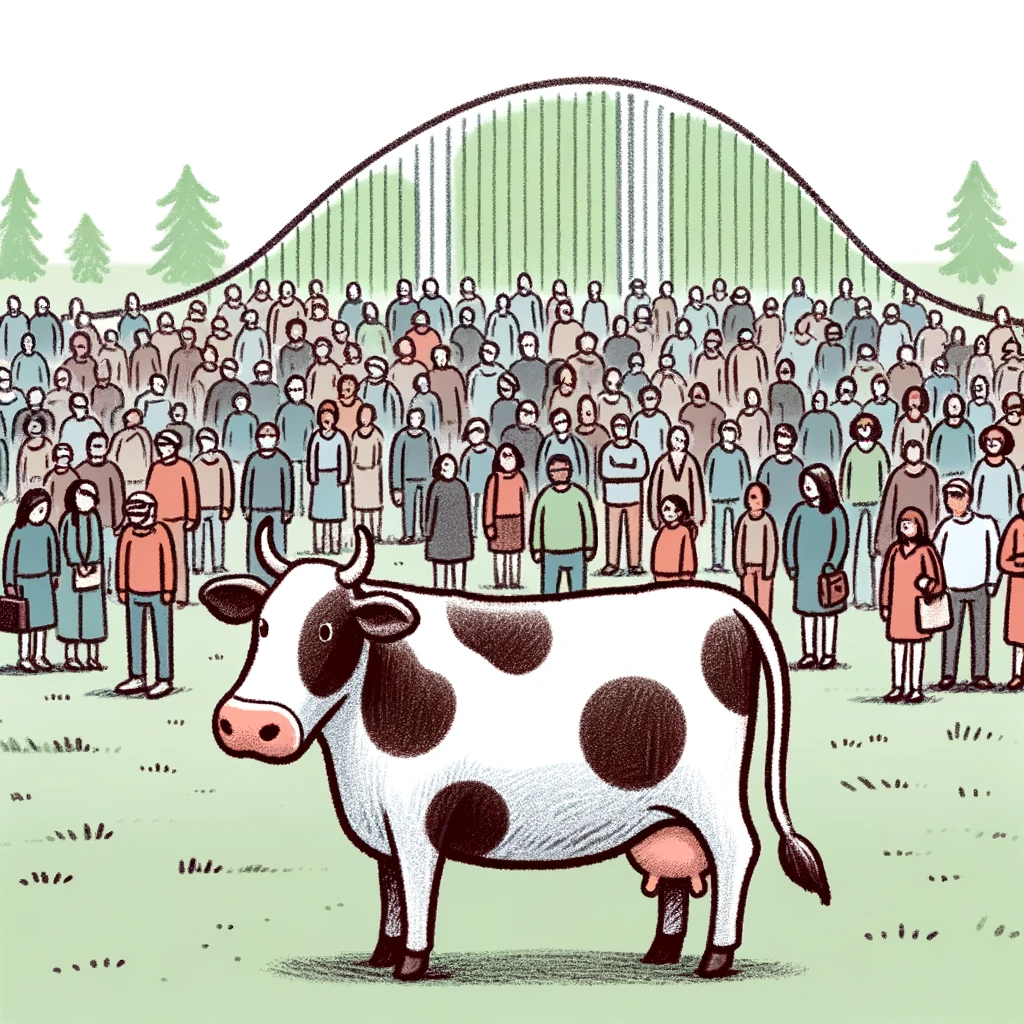
\includegraphics[width=0.5\textwidth]{figures/cow.png}
    \caption[The Wisdom of Crowds]{\textit{\textbf{The Wisdom of Crowds:}} The average of multiple noisy estimates of the weight of a cow is more accurate than any individual estimate}\label{fig:wisdomofcrowds}
\end{figure}

In this thesis, we will explore Canonical Correlation Analysis, a multiview learning method predicated on the assumption that different \gls{views} provide complementary information about latent variables. The following sections will establish a formal framework for representation learning and motivate the use of Canonical Correlation Analysis in harnessing complementary information from multiview data.

\section{Learning Representations: Definitions and Notation}

Suppose we have a sequence of vector-valued random variables $X\sps{i} \in \R^{D_i}$ for $i \in \{1, \dots, I \}$
We want to learn meaningful $K$-dimensional \gls{representations}
\begin{equation}
    \label{eq:general-form-of-representations}
    Z\sps{i} = f\sps{i}( X\sps{i}; \theta\sps{i}).
\end{equation}
For convenience, define $D = \sum_{i=1}^I D_i$ and $\theta = \left(\theta\sps{i}\right)_{i=1}^I$.
Without loss of generality take $D_1 \geq D_2 \geq \cdots \geq D_I$.
We will consistently use We will consistently use the superscript $(i)$ to denote the $i$-th view and not as an exponentiation operation.
$d \in [D_i]$ for dimensions of input variables;
and $l,k \in [K]$ for dimensions of \gls{representations} - i.e. to subscript dimensions of $Z\sps{i}, f\sps{i}$.
Later on we will introduce total number of samples $N$.

We denote the inner product between two vectors $a$ and $b$ as $\langle a, b \rangle$, which is defined as:
\begin{align}
\label{eq:inner-product}
\langle a, b \rangle = a^\top b = \sum_{i=1}^n a_i b_i
\end{align}
where $a_i$ and $b_i$ are the $i$-th elements of vectors $a$ and $b$, respectively, and $n$ is the dimension of the vectors.

The inner product is a measure of similarity between two vectors, with larger values indicating higher similarity. It is also related to the angle $\theta$ between the vectors, as shown in the following equation:
\begin{align}
\label{eq:inner-product-angle}
\langle a, b \rangle = |a| |b| \cos(\theta)
\end{align}
where $|a|$ and $|b|$ are the Euclidean norms (lengths) of vectors $a$ and $b$, respectively.

In this report, when the functions $f$ are linear, we will typically refer to $u_k$ as \gls{weights}, $Z_k = X_k u_k$ as \gls{representations} or \gls{latent variables} (noting that in the CCA literature they are sometimes referred to as canonical variables \citep{borga_learning_1998}), depending on the context.
We will sometimes consider a matrix $U = \left(u_1, \dots, u_K\right) \in \R^{D \times K}$ of \gls{weights}, and a matrix $Z = \left(Z_1, \dots, Z_K\right) \in \R^{N \times K}$ of representations.
We will refer to the Pearson correlation between features and their respective latent variable $\Corr(X\sps{i}_j, Z_k)$ as the \gls{loadings} of $X\sps{i}_j$ on $Z_k$ \citep{rosipal2005overview, alpert1972interpretation, borga_learning_1998}, noting that the same concept has also been referred to as structure correlations \citep{meredith1964canonical}.

%Covariance matrices
We will use the notation $\Sigma_{ij}=\Cov(X\sps{i}, X\sps{j})$ for the population \gls{covariance matrix} between the random variables associated with view $i$ and $j$. This \gls{covariance matrix} captures the relationships between variables from different views. Each element of this matrix, $\Sigma_{ij}(a,b)$, measures how much the $a$-th variable in view $i$ and the $b$-th variable in view $j$ change together, even though they belong to different views. A positive covariance indicates that the variables from different views tend to increase or decrease together, while a negative covariance indicates that they tend to move in opposite directions. These \glspl{covariance matrix} play a crucial role in multiview learning algorithms as they capture the inter-view relationships that the algorithms aim to leverage.

We will also use $\Sigma_{ii}= \Cov(X\sps{i})$ for the population \gls{covariance matrix} of the random variables associated with view $i$ with each other. This \gls{covariance matrix} captures the relationships between variables within the same view. Each element of this matrix, $\Sigma_{ii}(a,b)$, measures how much the $a$-th and $b$-th variables in view $i$ change together. A positive covariance indicates that the variables within the same view tend to increase or decrease together, while a negative covariance indicates that they tend to move in opposite directions. These within-view \glspl{covariance matrix} are essential for understanding the structure of the data in each view and are used in conjunction with the inter-view \glspl{covariance matrix} in multiview learning algorithms.

Many classical subspace learning algorithms can be formulated as Generalized Eigenvalue Problems (GEPs) constructed from \glspl{covariance matrix}. In the following subsection, we introduce the concept of GEPs and discuss their properties, which will be useful for understanding the optimization problems and solutions of these algorithms.

\subsection{Generalized Eigenvalue Problems in linear algebra}
A Generalized Eigenvalue Problem (GEP) is defined by two symmetric matrices $A,B\in \mathbb{R}^{D\times D}$ \citep{stewart_matrix_1990}\footnote{more generally, $A,B$ can be Hermitian, but we are only interested in the real case}.
They are usually characterized by the set of solutions to the equation:
\begin{align}
    \label{eq:igep}
    Au=\lambda Bu
\end{align}
with $\lambda \in \R, u \in \R^D$, called (generalized) eigenvalue and (generalized) eigenvector respectively.
When $B$ is positive definite, then the GEP becomes equivalent to an eigen-decomposition of the symmetric matrix $B^\mhalf A B^\mhalf$ \citep{ghojogh2019eigenvalue}.
In addition, one can find a basis of eigenvectors spanning $\R^D$.
We define a top-$K$ subspace to be one spanned by some set of eigenvectors {$u_1,\dots,u_K$} with the top-$K$ associated eigenvalues $\lambda_1 \geq \dots \geq \lambda_K$.
We say a matrix $U \in \R^{D \times K}$ defines a top-$K$ subspace if its columns span one.

\paragraph{Uniqueness}
In GEPs, the eigenvectors $u$ are not in general unique, but the generalized eigenvalues $1 \geq \lambda_1 \geq \lambda_2 \geq \dots \geq 0$ are unique \citep{mills1988calculation}.

\section{Classical Subspace Learning Algorithms}

\subsection{Principal Components Analysis}

Principal Components Analysis \citep{hotelling1933analysis} (\acrshort{pca}) is a classical method in unsupervised machine learning for representation learning.
It is widely used for dimensionality reduction and feature extraction.
The primary goal of \acrshort{pca} is to transform the original high-dimensional data into a new coordinate system defined by orthogonal axes, capturing the most relevant aspects of the data.

In \acrshort{pca}, the \gls{representations} are constrained to be linear transformations of the form:
\begin{equation}
    \label{eq:pca-linear-function-def}
    Z_k = X u_k,
\end{equation}
where $u_k$ are orthonormal basis vectors such that:
\begin{equation}
    \label{eq:pca-orthonormality-constraint}
    u_k^\top u_k = 1, \quad
    u_k^\top u_l = 0 \text{ for } k \neq l.
\end{equation}

The primary goal of \acrshort{pca} is to maximize the variance of the \gls{representations} \(Z_k\), finding the directions of maximal variance in the data.

\subsubsection{Optimization and Solution}
Mathematically, for the first principal component, this can be formulated as:

\begin{align}
    u_{\text{opt}} & = \underset{u}{\text{argmax}} \left( u^\top \Sigma u \right) \\
    \text{subject to:} \notag                                                     \\
    u^\top u& = 1 \notag
\end{align}

Where \(\Sigma = \mathbb{E}[X^\top X]\) is the population \gls{covariance matrix} of the single view data $X$.

To solve this constrained optimization problem, we can use the method of Lagrange multipliers. The key idea behind Lagrange multipliers is to transform a constrained optimization problem into an unconstrained one by incorporating the constraints into the objective function. The Lagrange multiplier, denoted by $\lambda$, can be thought of as a penalty for violating the constraint. By setting the Lagrange multiplier to a large enough value, we ensure that the optimal solution satisfies the constraint.

The Lagrangian function for the PCA optimization problem is constructed by adding the constraint multiplied by the Lagrange multiplier to the original objective function:

\begin{equation}
    f(u,\lambda) = u^\top \Sigma u + \lambda(1 - u^\top u),
\end{equation}
where \(\lambda\) is the Lagrange multiplier.

Intuitively, the first term in the Lagrangian represents the objective function (maximizing the variance), while the second term penalizes solutions that violate the constraint (unit norm). By finding the stationary points of the Lagrangian with respect to both $u$ and $\lambda$, we obtain the optimal solution that maximizes the variance while satisfying the unit norm constraint.

Differentiating the Lagrangian with respect to $u$ and setting it to zero yields the first-order conditions (which are necessary for optimality for the optimal $u$):
\begin{align}
\Sigma u & = \lambda u, \\
u^\top u & = 1.
\end{align}

\paragraph{Eigenvalue Problem}

This transforms the problem into an eigenvalue equation for the \gls{covariance matrix} \(\Sigma\), which can be efficiently solved using standard libraries such as scikit-learn \citep{pedregosa2011scikit}.

The first principal component therefore corresponds to the eigenvector associated with the largest eigenvalue \(\lambda\).
Subsequent components are the remaining eigenvectors ordered by their corresponding eigenvalues.

\subsubsection{Limitations}
There are three major limitations of \acrshort{pca} that are relevant to this thesis.

\begin{enumerate}
    \item \textbf{Scale Invariance}: as highlighted in the epigraph to this chapter, \acrshort{pca} is not scale invariant, meaning that the importance of a principal component can be disproportionately affected by the scale of the variables in the data. Variables measured at larger scales can dominate over those measured at smaller scales unless the data is normalized. This sensitivity to the scale of the data can lead to misleading directions that do not necessarily capture the most meaningful underlying structures.

    \item \textbf{Sparsity and Interpretability}: Although \acrshort{pca} reduces dimensionality by projecting the data onto new axes, the resulting principal components are linear combinations of \textit{all} the original features. This complex aggregation can make it difficult to interpret the components, especially when each component is influenced by many original variables. For this reason, sparse variants of \acrshort{pca} have been developed \citep{zou2006sparse,zou2018selective}, which aim to find sparse linear combinations of the original features; interpretable as a subset of the original features contributing to a significant proportion of the variance in the data.

    \item \textbf{Multiview Data Utilization}: \acrshort{pca} is primarily designed for analyzing a single dataset and does not naturally accommodate multiview data, where multiple independent sets of variables (views) describe the data. While it is possible to concatenate these \gls{views} into a single dataset prior to analysis, this approach does not take advantage of the potential interactions and complementary information across the views, which can be critical for more insightful analysis in applications such as image processing, bioinformatics, and social sciences.
\end{enumerate}

Nevertheless, \acrshort{pca} remains a popular tool in practice \citep{greenacre2022principal} and is a useful baseline for multiview learning methods, and we will use it as a point of comparison throughout this thesis.

\subsection{Partial Least Squares}

Given the inherent limitations of \acrshort{pca}, especially in handling multiview datasets where capturing interactive and complementary information between different data sources is crucial, Partial Least Squares (PLS) emerges as a potent alternative. PLS extends the principles of PCA to analyze two correlated \gls{views} simultaneously, optimizing for the shared covariance rather than variance within a single dataset. This approach makes PLS particularly valuable in multiview settings where the goal is to uncover the latent structures that explain the relationships between views.

Partial Least Squares (PLS) \citep{wold1975path} aims to maximize the shared covariance between two paired sets of data, referred to as \gls{views}. \acrshort{pls} can be seen as a generalization of \acrshort{pca}, where \acrshort{pca} becomes a special case when the two \gls{views} are identical.

\acrshort{pls} optimizes for the dot product between the \gls{representations} of two views, a measure of similarity.

\begin{align}
    \label{eq:dot-product}
    \langle X\sps{1}u^{(1)}, X\sps{2}u^{(2)}\rangle = |X\sps{1}u^{(1)}| |X\sps{2}u^{(2)}| \cos(\theta) = u\spsT{1} \Sigma_{12} u\sps{2}
\end{align}

Where $\theta$ is the angle between the two representations.
Much like for PCA, the \gls{representations} are constrained to be linear transformations of the form:

\begin{align}
    Z\sps{i} = X\sps{i} u\sps{i}
\end{align}

Where $u\sps{i}$ are orthonormal basis vectors such that:

\begin{align}
    u\spsT{i}u\sps{i} & = 1 \\
    u\spsT{i}u\sps{j} & = 0 \text{ for } i \neq j
\end{align}

\subsubsection{Optimization and Solution}

The constrained optimization problem for \acrshort{pls} can therefore be formulated as:

\begin{align}
    u\sps{1}_{\text{opt}} & = \underset{u\sps{1}}{\mathrm{argmax}} \{ u\spsT{1} \Sigma_{12} u\sps{2} \} \\
    \text{subject to:} \notag                                                                             \\
    u\spsT{1}u\sps{1}   & = 1 \notag                                                                    \\
    u\spsT{2}u\sps{2}   & = 1 \notag
\end{align}

The Lagrangian for this optimization problem once again integrates the constraints as penalties:

\begin{equation}
    f(u\sps{1}, \lambda) = u\spsT{1} \Sigma_{12} u\sps{2} + \lambda_1 (1 - u\spsT{1}u\sps{1}) + \lambda_2 (1 - u\spsT{2}u\sps{2})
\end{equation}

Upon deriving the first order conditions, we get:

\begin{align}
    \Sigma_{21} u\sps{1} & = \lambda_2 u\sps{2} \\
    \Sigma_{12} u\sps{2} & = \lambda_1 u\sps{1} \\
    u\spsT{1}u\sps{1}  & = 1                  \\
    u\spsT{2}u\sps{2}  & = 1
\end{align}

By substituting the constraint conditions into these equations, we find that \( \lambda_1 = \lambda_2 = \lambda \) by symmetry. Further simplification yields:

\begin{align}
    \Sigma_{21} \Sigma_{12} u\sps{2} & = \lambda^2 u\sps{2} \\
    \Sigma_{12} \Sigma_{21} u\sps{1} & = \lambda^2 u\sps{1}
\end{align}

\paragraph{Eigenvalue Problem}

Once again, we see that solving these equations will yield the \( u\sps{1} \) and \( u\sps{2} \) vectors as eigenvectors, this time of \( \Sigma_{12} \Sigma_{21} \) and \( \Sigma_{21} \Sigma_{12} \), respectively \citep{hoskuldsson1988pls}.

\paragraph{Generalized Eigenvalue Problem}

We can also represent the system of equations in matrix form as follows:

\begin{align}
    \begin{pmatrix}
        0           & \Sigma_{12} \\
        \Sigma_{21} & 0
    \end{pmatrix}
    \begin{pmatrix}
        u\sps{1} \\
        u\sps{2}
    \end{pmatrix}
    =
    \lambda
    I
    \begin{pmatrix}
        u\sps{1} \\
        u\sps{2}
    \end{pmatrix}
\end{align}

Which is of the form $A v = \lambda B v$. \acrshort{pls} is therefore also defined by the solution to a single generalized eigenvalue problem.

Given the notions of uniqueness in GEPs, the \gls{weights} $u$ are not in general unique but we can write the vector of generalized eigenvalues $(\lambda_1, \dots, \lambda_K)$ representing covariances as:

\begin{align}
    \label{eq:pls-vector-of-correlations-def}
    \PLS_K(X^{(1)},X^{(2)}) \defeq (\lambda_k)_{k=1}^K
\end{align}

\subsubsection{Limitations} 

Despite the advantages of \acrshort{pls} over \acrshort{pca} in handling multiview datasets, PLS has its own limitations that can impact its effectiveness in certain applications:
\begin{enumerate}
    \item \textbf{Scale Invariance}: Similar to \acrshort{pca}, \acrshort{pls} is not scale invariant. This means that the model's outcomes are affected by the scale of the features, potentially leading to biased \gls{weights} towards features with larger scale unless data is normalized.
    \item \textbf{Sparsity and Interpretability}: \acrshort{pls} does not inherently produce sparse models. The components derived from PLS are linear combinations of all input features, which can make the model difficult to interpret, particularly in high-dimensional contexts such as genomics or text processing. Sparse \acrshort{pls} has also been an active area of research \citep{chun2010sparse, witten2009penalized}.
\end{enumerate}

\subsection{Canonical Correlation Analysis}\label{sec:cca}

Canonical Correlation Analysis (\acrshort{cca}) is introduced as an advancement over \acrshort{pls}, designed to maximize the correlation instead of covariance between representations. This focus on correlation allows for a more nuanced understanding of the relationships between views, making \acrshort{cca} particularly useful in scenarios where the goal is to explore how \gls{views} relate on a normalized scale.

\acrshort{cca} achieves this by optimizing the cosine of the angle between the representations, thus normalizing the effect of the scale of the data:

\begin{align}
    \label{eq:cosine-similarity}
    \cos(\theta) = \frac{\langle X\sps{1}u^{(1)}, X\sps{2}u^{(2)}\rangle}{|X\sps{1}u^{(1)}| |X\sps{2}u^{(2)}|}= \frac{u\spsT{1}\Sigma_{12}u\sps{2}}{|X\sps{1}u^{(1)}| |X\sps{2}u^{(2)}|}
\end{align}
By focusing on correlation, \acrshort{cca} normalizes the contributions of each variable, ensuring that the analysis is not unduly influenced by the magnitude of the data. This normalization is particularly valuable in multiview settings where the scales of the data sources may differ significantly.

\subsubsection{Optimization and Solution}

If we constrain the norms of the representations to be equal to 1, i.e., $|X\sps{1}u^{(1)}|=|X\sps{2}u^{(2)}|=1$, then maximizing the cosine similarity is equivalent to maximizing the numerator $u\spsT{1}\Sigma_{12}u\sps{2}$. This leads to the following constrained optimization problem:

\begin{align}
    & u_{\text{opt}}=\underset{u}{\mathrm{argmax}}\{ u\spsT{1}X\spsT{1}X\sps{2}u\sps{2} \} \\
    & \text{subject to:} \notag                                                                \\
    & u\spsT{1}\Sigma_{11}u\sps{1}=1 \notag                                                  \\
    & u\spsT{2}\Sigma_{22}u\sps{2}=1 \notag
\end{align}

By focusing on correlation and imposing unit norm constraints on the representations, \acrshort{cca} normalizes the contributions of each variable, ensuring that the analysis is not unduly influenced by the magnitude of the data. This normalization is particularly valuable in multiview settings where the scales of the data sources may differ significantly.

Although non-convex, numerous methods exist for solving the \acrshort{cca} problem, including eigendecomposition and generalized eigendecomposition solvers \citep{uurtio2017tutorial} and block coordinate descent via alternating least squares regressions \citep{golub1995canonical,sun2008least}.

The first-order conditions derived in the same manner as the \acrshort{pls} case are:

\begin{align}
    \label{CCA:FOCs}
    & \Sigma_{21}u\sps{1}=\lambda\sps{2} \Sigma_{22}u\sps{2} \\
    & \Sigma_{12}u\sps{2}=\lambda\sps{1} \Sigma_{11}u\sps{1} \\
    & u\spsT{1}\Sigma_{11}u\sps{1}=1                       \\
    & u\spsT{2}\Sigma_{22}u\sps{2}=1
\end{align}

\paragraph{Eigenvalue Problems}

Substituting the second two conditions into the first two, we get \(\lambda\sps{1}=\lambda\sps{2}=\lambda\). Finally, substituting the first two conditions into each other, we find the eigenvalue problems:

\begin{align}\label{eq:cca-eigenvalue-problems}
    & \Sigma_{11}^{-1}\Sigma_{12}\Sigma_{22}^{-1}\Sigma_{21}u\sps{1}=\lambda^2u\sps{1} \\
    & \Sigma_{22}^{-1}\Sigma_{21}\Sigma_{11}^{-1}\Sigma_{12}u\sps{2}=\lambda^2u\sps{2}
\end{align}

An alternative form of the \acrshort{cca} problem can be developed by reparameterizing \(u\sps{i*}=\Sigma_{ii}^{-\frac{1}{2}}u\sps{i}\). The optimization problem then becomes:

\begin{align}\label{eq:cca-reparameterized}
    & u_{\text{opt}}=\underset{u}{\mathrm{argmax}}\{ u\spsT{1}\Sigma_{11}^{-\frac{1}{2}}\Sigma_{12}\Sigma_{22}^{-\frac{1}{2}}u\sps{2} \} \\
    & \text{subject to:} \notag                                                                                                            \\
    & u\spsT{1}u\sps{1}=1 \notag                                                                                                         \\
    & u\spsT{2}u\sps{2}=1 \notag
\end{align}

This reparameterized form will later underpin Deep Canonical Correlation Analysis (\acrshort{dcca}) through the matrix $T=\Sigma_{11}^{-\frac{1}{2}}\Sigma_{12}\Sigma_{22}^{-\frac{1}{2}}$.
This form also shows that \acrshort{pls} and \acrshort{cca} can be made equivalent by whitening the data matrices before constructing the \glspl{covariance matrix}.
When the number of features exceeds the number of samples (\(p>n\)), \acrshort{cca} becomes degenerate because the within-view \glspl{covariance matrix} cannot be inverted—contrasting with \acrshort{pls}, which is always computable.

\paragraph{Generalized Eigenvalue Problem}

We can also represent the system of equations in equation~\ref{CCA:FOCs} as a matrix equation:

\begin{align}
    \begin{pmatrix}
        0           & \Sigma_{12} \\
        \Sigma_{21} & 0
    \end{pmatrix}
    \begin{pmatrix}
        u\sps{1} \\
        u\sps{2}
    \end{pmatrix}
    =
    \lambda
    \begin{pmatrix}
        \Sigma_{11} & 0           \\
        0           & \Sigma_{22}
    \end{pmatrix}
    \begin{pmatrix}
        u\sps{1} \\
        u\sps{2}
    \end{pmatrix}
\end{align}

Which is once again of the form $A u = \lambda B u$. \acrshort{cca}, like \acrshort{pls}, is therefore also defined by the solution to a single generalized eigenvalue problem.

\paragraph{Canonical Correlations}
In the case of \acrshort{cca}, the generalized eigenvalues $\lambda$ are generally called canonical correlations \citep{hotelling1935canonical, hotelling1992relations}.
Given the notions of uniqueness in GEPs, the \gls{weights} $u$ are not in general unique but we can write the vector of generalized eigenvalues or canonical correlations as:
\begin{align}
    \label{eq:cca-vector-of-correlations-def}\small
    \CCA_K(X^{(1)},X^{(2)}) \defeq (\rho_k)_{k=1}^K
\end{align}

\subsubsection{Limitations}

A major limitation of \acrshort{cca} is revealed by the forms in equations \ref{eq:cca-eigenvalue-problems} and equation~\ref{eq:cca-reparameterized}; \acrshort{cca} in general requires the inversion of  \glspl{covariance matrix}, which is computationally expensive, potentially numerically unstable, and impossible when the number of features exceeds the number of samples such that the  \glspl{covariance matrix} are not full rank.

\subsection{Multiview \acrshort{cca}}

Multiview \acrshort{cca} (\acrshort{mcca}) is an extension of \acrshort{cca} that handles more than two \gls{views} simultaneously. Given $I$ \gls{views} $X\sps{1}, \dots, X\sps{i}$, the goal of MCCA is to find a set of directions $u\sps{1}, \dots, u\sps{i}$ that maximize the sum of pairwise correlations between the projections of the \gls{views} onto these directions.
\subsubsection{Optimization and Solution}

The optimization problem for \acrshort{mcca} can be formulated as follows:
\begin{align}
    & u_{\text{opt}} = \underset{u}{\mathrm{argmax}} \sum_{i=1}^{I} \sum_{j=1, j \neq i}^{I} u\spsT{i} \Sigma_{ij} u\sps{j} \\
    & \text{subject to:} \notag                                                                                               \\
    & \sum_{i=1}^{I} u\spsT{i} \Sigma_{ii} u\sps{i} = 1 \notag
\end{align}

\paragraph{Generalized Eigenvalue Problem}

The MCCA optimization problem can be solved by formulating it as a generalized eigenvalue problem (GEP). The GEP for MCCA can be written in matrix form as follows:

\begin{align}
    \small
    \underbrace{\begin{pmatrix}
        0           & \Sigma_{12} & \cdots & \Sigma_{1I} \\
        \Sigma_{21} & 0           & \cdots & \Sigma_{2I} \\
        \vdots      & \vdots      & \ddots & \vdots      \\
        \Sigma_{I1} & \Sigma_{I2} & \cdots & 0
    \end{pmatrix}}_{A}
    \begin{pmatrix}
        u\sps{1} \\
        u\sps{2} \\
        \vdots   \\
        u\sps{I}
    \end{pmatrix}
    =
    \lambda
    \underbrace{\begin{pmatrix}
        \Sigma_{11} & 0           & \cdots & 0           \\
        0           & \Sigma_{22} & \cdots & 0           \\
        \vdots      & \vdots      & \ddots & \vdots      \\
        0           & 0           & \cdots & \Sigma_{II}
    \end{pmatrix}}_{B}
    \begin{pmatrix}
        u\sps{1} \\
        u\sps{2} \\
        \vdots   \\
        u\sps{I}
    \end{pmatrix}.
\end{align}

The matrix $A$ contains the cross-covariance matrices between the views, while the matrix $B$ is a block diagonal matrix containing the within-view covariance matrices. The solution to the GEP gives the optimal directions $u\sps{1}, \dots, u\sps{I}$ and the corresponding generalized eigenvalues $\lambda$.

\paragraph{Unified Framework}

The GEP formulation of MCCA can be further generalized to include ridge regularization, which helps stabilize the solution when the  \glspl{covariance matrix} are ill-conditioned. This leads to a unified framework that encompasses both CCA and its ridge-regularized extensions.

Let $A,B_\alpha \in \R^{D \times D}$ be block matrices defined as follows:
\begin{align}
    A_{ij} &= \Cov(X\sps{i}, X\sps{j}) \text{ for } i \neq j, \\
    B_{\alpha,ii} &= \alpha_i I_{D\sps{i}} + (1-\alpha_i) \Var(X\sps{i}),
\end{align}
where $\alpha \in [0,1]^I$ is a vector of ridge penalty parameters. Setting $\alpha_i = 0 \: \forall i$ recovers the standard CCA, while $\alpha_i = 1 \: \forall i$ yields the PLS solution.

In the case of standard CCA (i.e., $\alpha=0$), we can define the MCCA correlation vector as:
\begin{align}\label{eq:MCCA}
    \MCCA_K(X\sps{1},\dots,X\sps{I}) = (\lambda_1, \dots, \lambda_K),
\end{align}
where $\lambda_1, \dots, \lambda_K$ are the top-$K$ generalized eigenvalues. These eigenvalues represent the average of the top-$K$ correlations between each pair of views.

\subsection{Linear Discriminant Analysis LDA}

Linear Discriminant Analysis (LDA) can be viewed as a special case of Canonical Correlation Analysis (CCA) where \(X^{(2)}\) is a one-hot encoded matrix representing the class labels.
This allows us to draw a connection between the unsupervised learning framework of \acrshort{cca} and the supervised framework of LDA\citep{balakrishnama1998linear,riffenburgh1957linear}, thus expanding the understanding of both algorithms.

\textbf{Intuition:} In LDA, the aim is to find a lower-dimensional subspace where the classes are maximally separated. This objective can be viewed through the lens of \acrshort{cca}, where the optimal directions \(u^{(1)}\) and \(u^{(2)}\) in the original and one-hot encoded spaces aim to maximize correlation. In the LDA context, \(u^{(1)}\) would maximize the separation between classes.

\subsubsection{Optimization and Solution}

Mathematically, LDA is reduced to solving a generalized eigenvalue problem involving the between-class scatter matrix \(S_B\) and the within-class scatter matrix \(S_W\):

\[
    \hat{S_B} = \sum_{i=1}^{c} n_i (\mu_i - \mu)(\mu_i - \mu)\top
\]

\[
    \hat{S_W} = \sum_{i=1}^{c} \sum_{x \in X_i} (x - \mu_i)(x - \mu_i)\top
\]

\textbf{Connection to \acrshort{cca}:} When \(X^{(2)}\) is the one-hot encoded matrix of class labels, the \acrshort{cca} problem effectively tries to maximize the correlation between the feature vectors and their corresponding labels.
This turns out to be equivalent to maximizing the between-class variance in LDA while minimizing the within-class variance.
Thus, LDA can be thought of as a constrained form of \acrshort{cca}, tailored to classification tasks.

This perspective unifies the two algorithms and shows that the core objective—finding meaningful relationships or directions in the data—is shared between both \acrshort{cca} and LDA.

\subsection{Sample Covariance and Population Covariance}
In the previous sections, the methods were described in terms of population  \glspl{covariance matrix} such as \(\Sigma_{11}=\mathbb{E}[X\spsT{1} X\sps{1}]\), \(\Sigma_{22}=\mathbb{E}[X\spsT{2} X\sps{2}]\), and \(\Sigma_{12}=\mathbb{E}[X\spsT{1} X\sps{2}]\).
These population covariances assume an underlying probability distribution from which the data are drawn.

\textbf{Sample Covariance:} In practical settings, we often do not have access to the entire population but only to a sample. Hence, we can use the Sample Average Approximation to estimate these covariances:

\[
    \hat{\Sigma}\sps{12} = \frac{1}{b-1} \bar{\mathbf{X}\sps{1}} \bar{\mathbf{X}\sps{2}}\top
\]

Here, \(b\) denotes the size of the minibatch, and \(\mathbf{X}\sps{1} \in \mathbb{R}^{D_1 \times b}\) and \(\mathbf{X}\sps{2} \in \mathbb{R}^{D_2 \times b}\) are the data matrices for the samples from \(X\sps{1}\) and \(X\sps{2}\), respectively. The bar over \(\mathbf{X}\sps{1}\) and \(\mathbf{X}\sps{2}\) signifies that these are centered versions of the matrices, i.e., the mean has been subtracted from each column.
For the ease of both reader and writer, we will drop the bars for the remainder of the thesis and assume that all data matrices are centered without loss of generality.

\textbf{Practical Implications:} Using \glspl{sample covariance matrix} introduces some estimation error but allows us to apply the methods in real-world scenarios where population-level data are unattainable.
Additionally, the use of minibatches (chunks of data) in later chapters provides a computationally efficient way to estimate these covariances in large-scale problems, at the cost of some additional statistical noise.

\textbf{Connection to Previous Methods:} The use of \glspl{sample covariance matrix} is directly applicable to algorithms like \acrshort{cca} and LDA. When replacing the population covariances \(\Sigma\sps{ij}\) with sample estimates, the optimization problems remain structurally similar but are solved using the sample data.

This dual perspective—considering both population and sample covariance matrices—enables a more robust and flexible approach to the methods discussed, bridging the gap between theoretical analysis and practical application.
It will be particularly useful in the context of chapter \ref{ch:loadings} where we will use population variables as ground truth while estimating the models using sample data.


\section{Practical Frameworks for Evaluating Multiview Learning Methods}

At this point, we have introduced the theoretical foundations of multiview learning, and a number of classical representation learning algorithms including \acrshort{cca} and its variants.
However, it is not yet clear how we should evaluate these methods in practice.
In this section, we compare the machine learning and the statistical approach of permutation testing.
These two approaches are not mutually exclusive, and statistical learning theory has emerged as a unifying framework for both perspectives \citep{vapnik1999nature, hastie2009elements}.

\subsection{Permutation Testing}

\begin{figure}
    \centering
    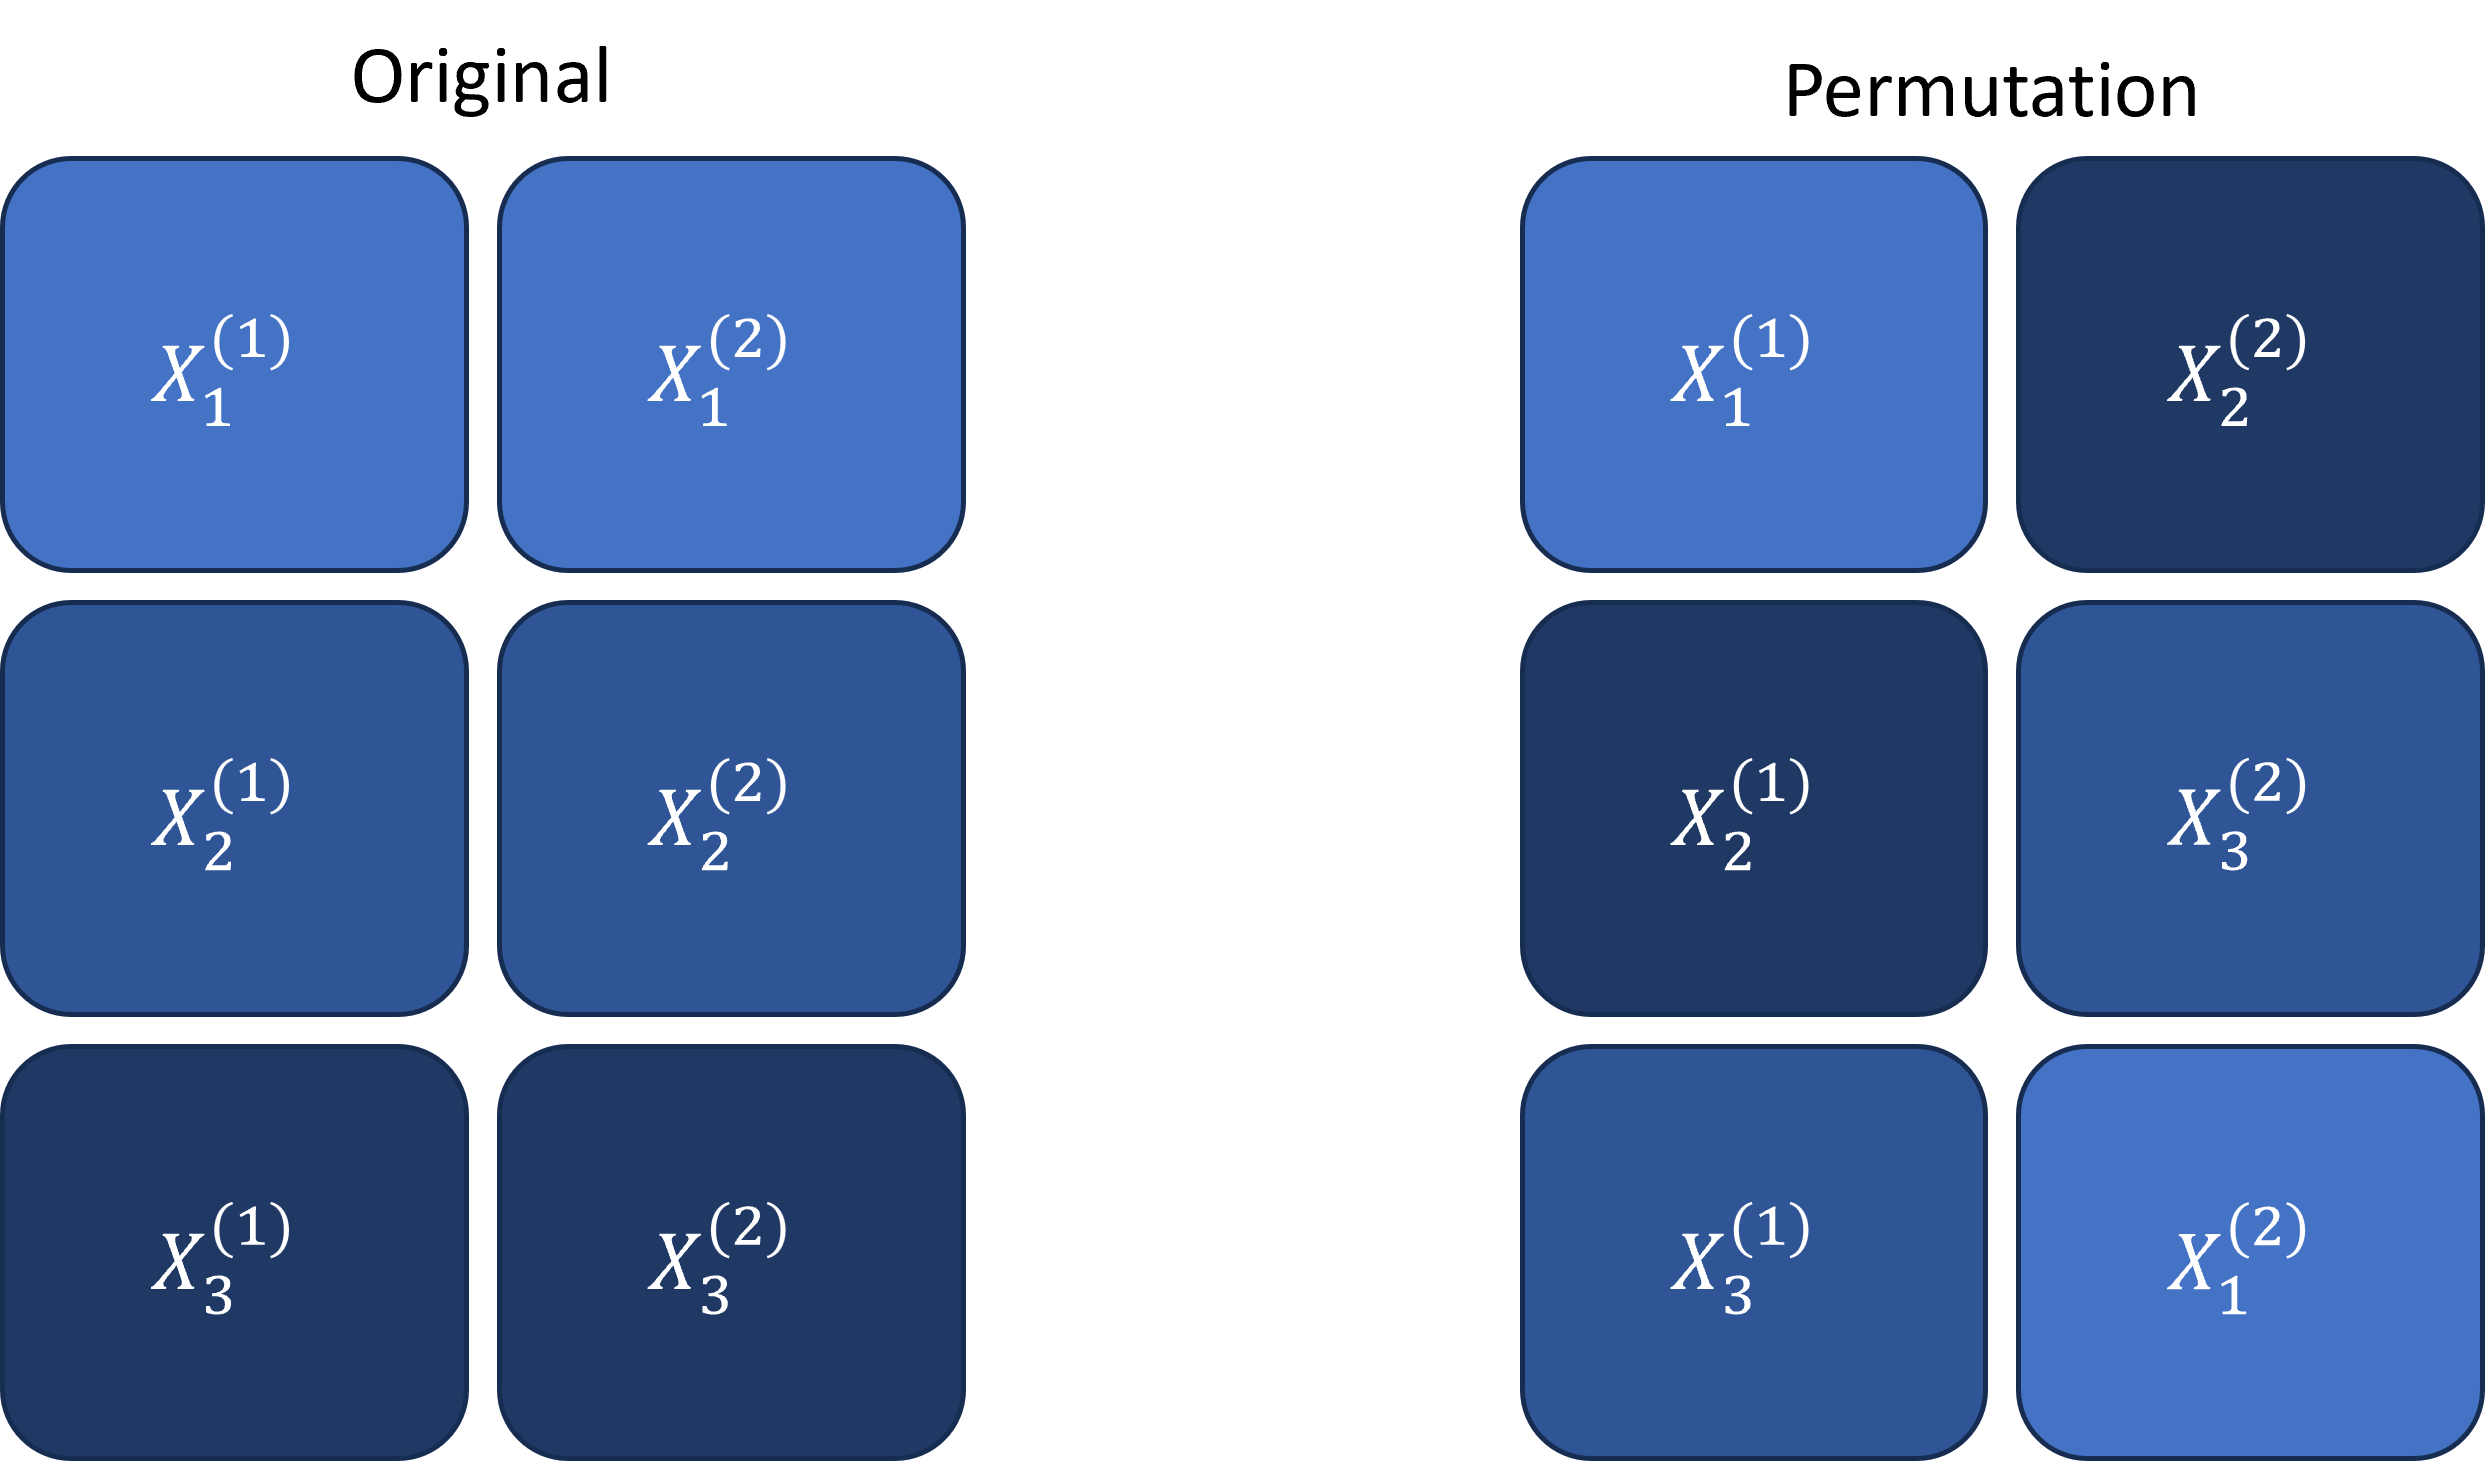
\includegraphics[width=0.8\textwidth]{figures/permutation_test.png}
    \caption{Schematic of the permutation testing procedure. The original data are randomly shuffled, and the model is retrained on the shuffled data. This process is repeated multiple times, and the model's performance on the original data is compared to the distribution of performances on the shuffled data.}
    \label{fig:statistical-inference}
\end{figure}

Permutation testing offers a robust way to evaluate the significance of the results obtained by multiview learning methods and, for a single component, is a relatively simple process \citep{winkler2020permutation}.
As illustrated in Figure~\ref{fig:statistical-inference}, the \gls{views} are randomly and separately shuffled, and the model is then trained and tested on this permuted data.
This process is repeated multiple times, generating a distribution of performance metrics under the null hypothesis, where there is no relationship between the views.
The actual performance of the model on the unshuffled data is then compared to this distribution.
If the actual performance is significantly better than the permuted performance, it suggests that the model is capturing meaningful relationships in the data.

\subsection{Machine Learning}

\begin{figure}
    \centering
    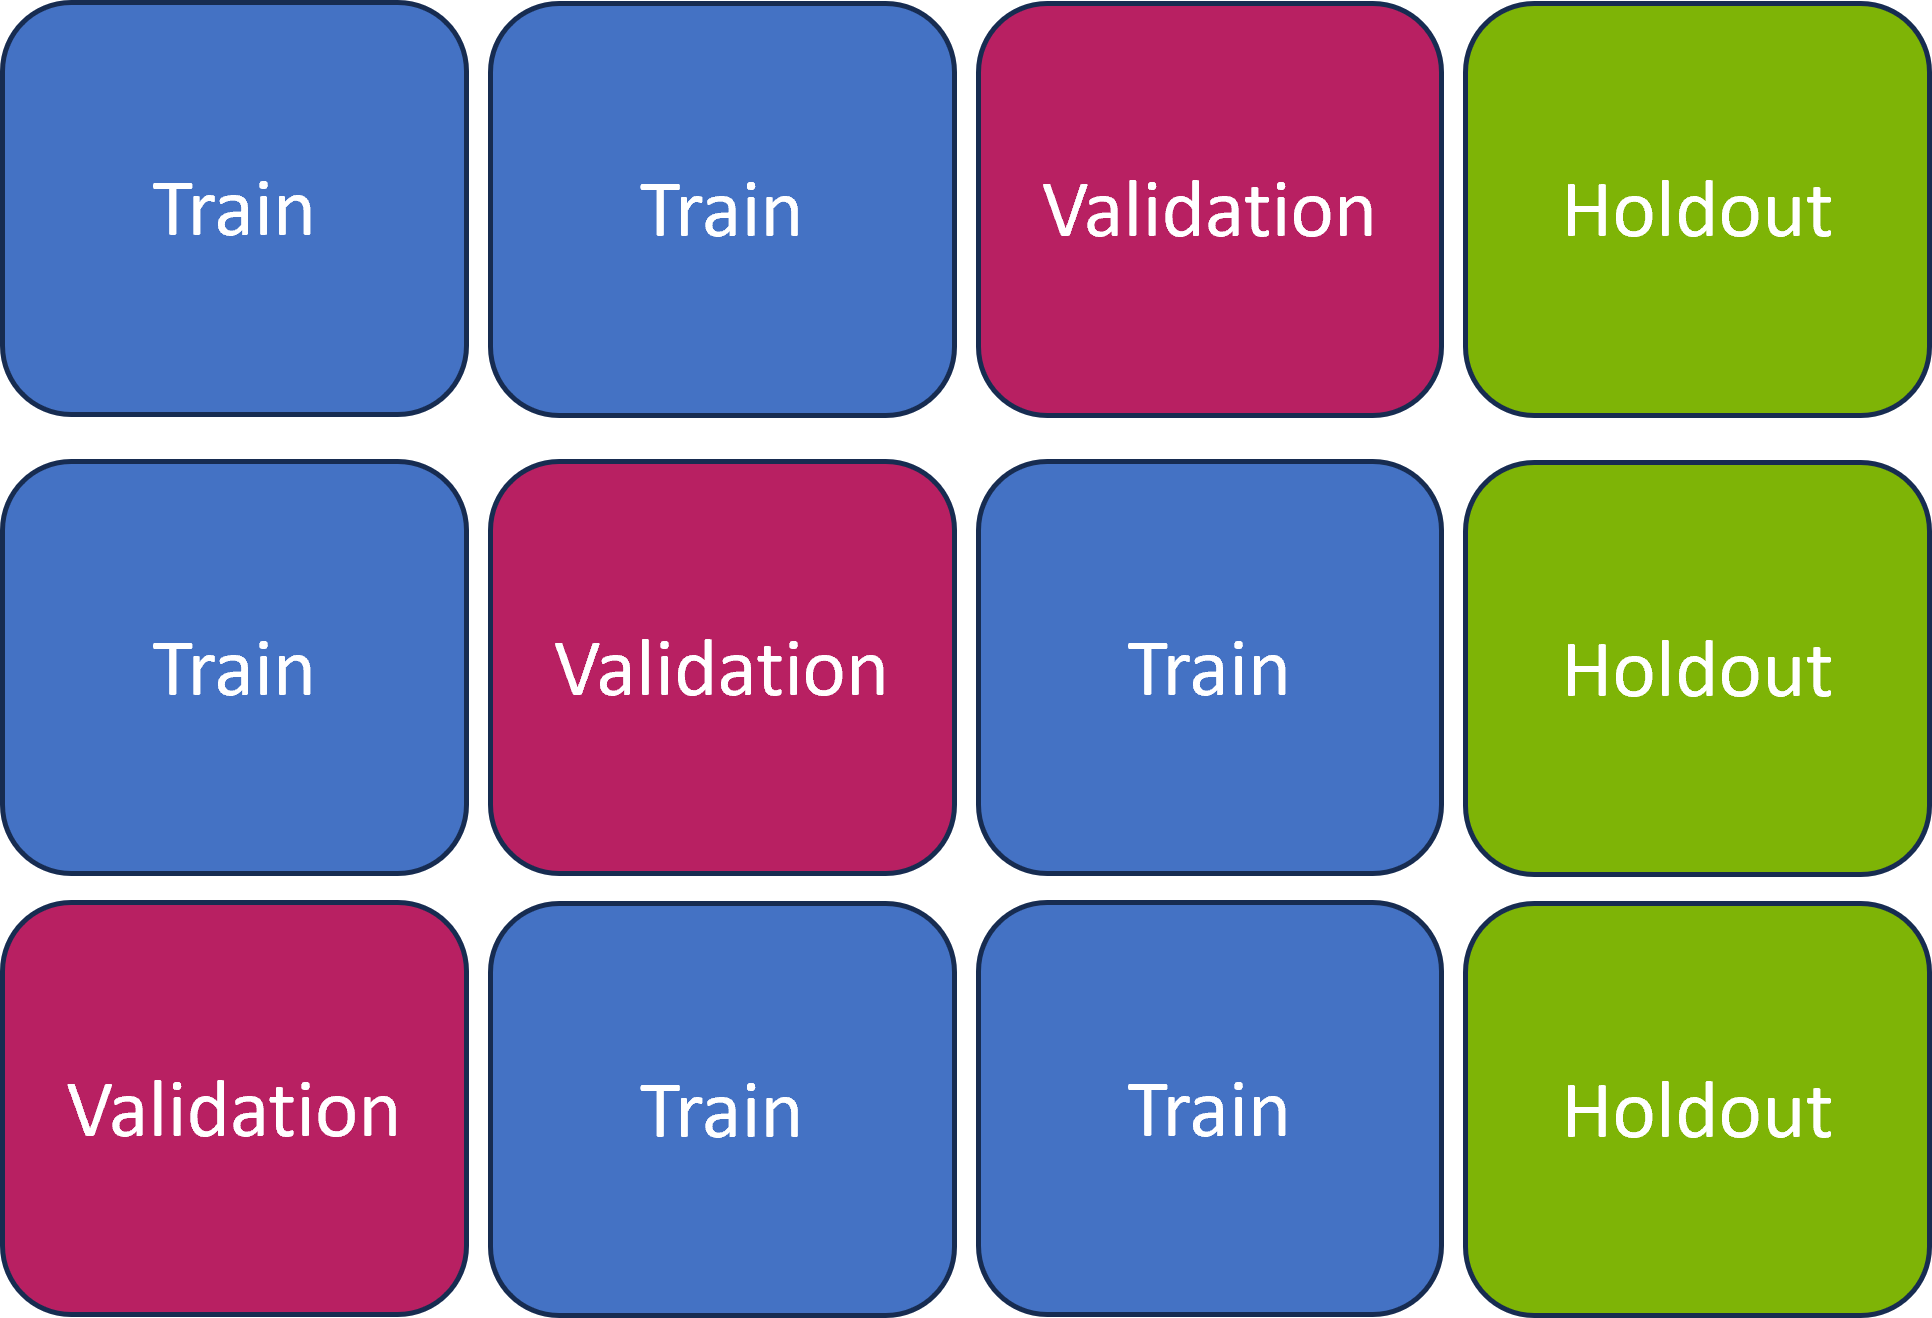
\includegraphics[width=0.8\textwidth]{figures/cross-validation.png}
    \caption{Schematic of the cross-validation procedure. The original data are partitioned into training and test sets. In cross-validation, the training set is further partitioned into training and validation sets. The model is trained on the training set and evaluated on the validation set for different parameter values. The parameter value with the best performance on the validation set is selected, and the model is retrained on the entire training set. The final model is evaluated on the single test or holdout set.}
    \label{fig:machine-learning}
\end{figure}

The machine learning approach to evaluating multiview learning methods is to use a holdout or test set to estimate the out-of-sample performance of the model.
Within the training set, where necessary, cross-validation is used to select the best model hyperparameters.
Cross-validation involves partitioning the training set into training and validation sets, training the model on the training set, and evaluating the model on the validation set.
When this is performed for multiple subsets of the training set, it is referred to as \(k\)-fold cross-validation as illustrated in figure \ref{fig:machine-learning}.
The model hyperparameters are then selected based on the performance across the validation sets.
The model is then retrained on the entire training set using the best hyperparameters, and evaluated on the test set.

In this thesis, we will use the machine learning approach throughout.
This is because in scaling up to large datasets, permutation testing becomes computationally intractable.
This is because permutation testing requires retraining the model multiple times on the permuted data.
This comes at the cost of only being able to evaluate models with a point estimate of performance, rather than a distribution.

\subsection{Components and Subspaces in CCA}

\subsubsection{Eigenvalue Problems in CCA}

While our focus so far has primarily been on the top-1 eigenvector-eigenvalue pair, it's important to note that the methodology also extends to the top-k subspace problem.
This broader approach involves identifying the top-k eigenvectors and their corresponding eigenvalues.

\subsubsection{Addressing the Top-k Problem}

Transitioning from a focus on the top-1 component to exploring the top-k subspace introduces additional complexities. One common method to solve the top-k problem is to identify the top-1 component and then apply a deflation process to find subsequent orthogonal components.
Deflation involves removing the top-1 component from the data and then repeating the process to find the next top-1 component. This process is repeated until the desired number of components is found.
For instance, Hotelling's Deflation \citep{hotelling1933analysis} involves removing the top-1 component from the data, while Projection Deflation \citep{mackey2008deflation} involves projecting the data onto the orthogonal complement of the top-1 component.
Different deflation methods enforce different forms of orthogonality, which can impact the resulting components and their interpretation, particularly when the first component is not a true eigenvector.

\subsubsection{Non-Uniqueness of Components}

Furthermore, non-uniqueness is a significant challenge in representation learning, particularly when eigenvectors have repeated eigenvalues. Imagine a scenario where the top-1 eigenvalue is repeated \(k\) times. In this case, there are \(k\) possible eigenvectors that can be associated with the top-1 eigenvalue. While this is unlikely to occur in practice, the eigenvalues can in practice be very close to each other, leading to numerical instability and non-uniqueness in the components. Particularly true in cross-validation settings, this non-uniqueness can lead to instability in the components, complicating their interpretation and comparison.
For example, the top-1 component in one analysis might be the second component in another analysis, making it difficult to compare the results.

This non-uniqueness also has a grounding in the probabilistic perspectives on PCA and CCA (introduced in chapter \ref{ch:loadings}), where the latent variables are considered unique only up to a rotation.
This perspective further reinforces the subspace approach, emphasizing the identification of a subspace rather than specific directions within it.

\paragraph{Thesis Approach: Concentrating on the Top-1 Component}

In this thesis, we focus on the top-1 component in CCA to align with and facilitate comparison with typical componentwise studies in brain-behavior research.
This choice is driven by the complexity associated with the top-k problem and the variety of methods available to address it.
Under the assumption of a significant eigengap\footnote{An `eigengap' refers to the difference in magnitude between consecutive eigenvalues in an eigenvalue problem. A significant eigengap between the first and second eigenvalues suggests that the first eigenvalue (and its corresponding eigenvector) is distinctly more significant than the next, lending credence to its uniqueness and importance.}, the first component can be considered equivalent to the top-1 subspace.
This equivalence allows for a clear and interpretable analysis, making the top-1 subspace a straightforward and reliable choice for studying multivariate data.
It is important to note that while we focus on the top-1 component, the later sections of the thesis introduce a method for simultaneously solving the complete subspace, addressing broader subspace analyses.


\section{Multiview Learning in Neuroimaging}

Finally, we review important applications of multiview learning from the literature in neuroimaging, which will be our reference in chapters \ref{ch:als} and \ref{ch:loadings}.

\subsection{Multiview Data in Neuroscience and Genetics}

In neuroscience and genetics, two specific types of multiview studies are particularly relevant to this thesis: brain-behavior studies and imaging-genetics.
Both involve the integration of data from multiple sources, offering rich insights into complex phenomena.

Brain-behavior studies typically involve pairing neuroimaging data, such as that obtained from Structural MRI (sMRI) or Functional MRI (fMRI), with non-imaging data like responses from questionnaires, cognitive test results, and other behavioral assessments.
sMRI provides detailed anatomical brain images, essential for understanding brain structure and neurological disorders \citep{kanai2011structural}, while fMRI focuses on brain function by mapping activity during cognitive tasks \citep{miranda2021systematic}.
The integration of these imaging techniques with behavioral data offers a comprehensive view of how brain structures and functions correlate with behavioral and cognitive patterns \citep{rypma2001age,genon2022linking}.

Imaging-Genetics, another critical multiview approach, combines neuroimaging data with genetics and omics information \citep{le2008sparse}.
This interdisciplinary field seeks to understand the genetic influences on brain structure and function, thereby illuminating the genetic basis of neuropsychiatric disorders and cognitive traits \citep{bogdan2017imaging}.
Studies in this area can explore how specific genetic variations correlate with differences in brain morphology or activity patterns observed in neuroimaging \citep{liu2014review}.

Together, these multiview approaches are fundamental in advancing our understanding of the brain's structure, function, and its interactions with genetic and behavioral factors.
They represent key applications of SSL in neuroscience and genetics, providing comprehensive insights that underpin developments in these fields.

\subsection{Applications of Multiview Learning in Neuroimaging}

There have been a number of applications of \acrshort{cca} and related methods to multiview problems in neuroimaging.
Using resting state fMRI data, modes of correlation have been found that relate to differences in sex and age relating to drug and alcohol abuse, depression and self harm \citep{mihalik2019brain}.
A similar mode relating to `positive-negative' wellbeing has been found across studies \citep{smith2015positive} suggesting that mental wellbeing has a relationship (though not necessarily causally) with functional connectivity between networks in the brain.
Later in this dissertation we will replicate and build on the findings from this paper by using regularised and non-linear \acrshort{cca} methods.
Owing to the high dimensionality of neuroimaging data, regularisation has been a particular focus of multiview learning in neuroimaging. \citet{mihalik2022canonical} reviews the application of \acrshort{cca} to neuroimaging data and highlights the importance of regularisation in this context. \citet{bilenko2016pyrcca} 
CCA has also been used as a preprocessing step in order to identify groups of subjects in the latent variable space.

In particular, \acrshort{cca} and clustering have been used to identify depression using fMRI data \citep{dinga2019evaluating,drysdale2017resting}.
CCA has also been used in the manner we described to denoise two \gls{views} of a dataset such as separate measures of neuroimaging data \citep{zhuang2020technical} to remove artefacts.
Deep \acrshort{cca} has recently been used to extract features for the diagnosis of schizophrenia\citep{qi2016deep}.

\section{Conclusion}

In this chapter, we have provided a comprehensive overview of multiview learning, with a particular focus on its applications in neuroimaging and genetics. We have discussed the fundamental concepts and methods in multiview learning, such as Canonical Correlation Analysis (CCA), Partial Least Squares (PLS), and their variants, highlighting their strengths and limitations.

The review has emphasized the importance of regularization techniques in high-dimensional settings, as well as the challenges associated with interpreting the resulting components. We have also touched upon the need for efficient algorithms that can handle large-scale datasets, and the potential of non-linear extensions of CCA and joint embedding self-supervised learning approaches.

Furthermore, we have discussed the practical frameworks for evaluating multiview learning methods, comparing the traditional statistical approach of permutation testing with the machine learning approach of cross-validation and holdout testing. We have also considered the complexities of identifying and interpreting top-k subspaces in CCA, and the reasons for focusing on the top-1 component in this thesis.

The applications of multiview learning in neuroimaging and genetics have been highlighted, with a particular emphasis on brain-behavior studies and imaging-genetics. These studies have demonstrated the potential of multiview learning in uncovering the complex relationships between brain structure, function, genetics, and behavior, thereby advancing our understanding of neurological disorders and cognitive traits.

Despite the significant progress made in multiview learning, several challenges remain. These include the need for more interpretable and regularized methods, particularly in high-dimensional settings, the development of efficient algorithms for handling large-scale datasets, and the extension of CCA to non-linear and deep learning-based approaches.

In the following chapters, this thesis aims to address these challenges by proposing novel methods and techniques for multiview learning. We will explore regularized and interpretable extensions of CCA, develop efficient algorithms for high-dimensional data, and investigate the potential of deep learning-based approaches for multiview learning. By tackling these challenges, we hope to contribute to the advancement of multiview learning and its applications in neuroimaging, genetics, and beyond.
